\begin{figure}

\centering

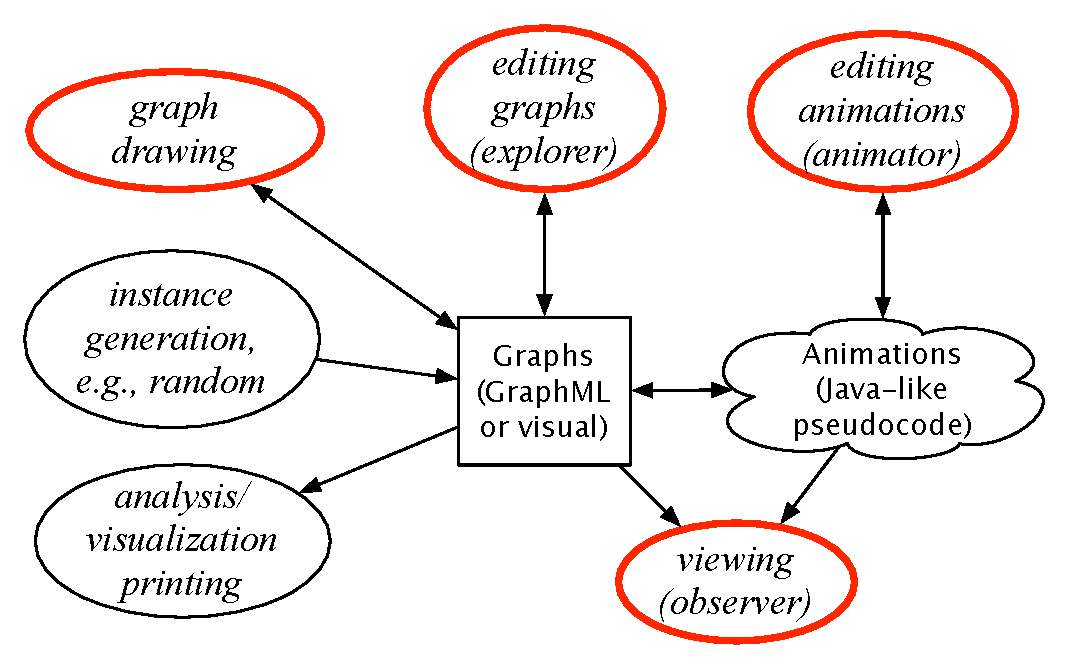
\includegraphics[width=\columnwidth]{X_overview_diagram}

\caption{Illustration of Galant design and functionality. Arrows indicate
  data flow. All functions, shown as ovals can be performed easily outside of
Galant. The ones with thick red borders are part of current Galant
functionality.}

\label{fig:overview_diagram}
\end{figure}

% [Last modified: 2013 06 25 at 16:04:45 GMT]


Fig.~\ref{fig:overview_diagram} gives an overview of Galant functionality.
A graphical user interface (GUI) allows the user to edit both graphs and
algorithm animations, either loaded as already existing files or newly
created. At any point, the user can apply a selected animation to a selected
graph for viewing.
The animation program runs to completion and compiles a sequence of states (steps),
each essentially a snapshot at a developer-defined break point.
The user can then navigate the animation forward or backward one step at a time.

When editing a graph the user can create vertices and edges by clicking and/or
moving the mouse, and can move vertices by dragging the mouse.
There is also an interface for specifying labels, weights and colors for both
edges and vertices.
A preferences panel allows the user to select font size for labels and a
variety of other options.
Any changes to a graph are also reflected in a text (GraphML) representation
of the graph, which can also be edited directly. Naturally the GraphML
representation can also be created or edited externally: by a random or
structured graph generator, by translation from another format, by directly
editing the GraphML or by invoking a separate graph editor.
Galant has a built-in force-directed drawing program 
(the one reported by Hu~\cite{2006-Mathematica-Hu}) to position nodes
automatically if so desired.
Other drawing programs, such as those provided by GraphViz~\cite{GraphViz}
and the huge body of research carried on by the graph drawing community~\cite{graph_drawing},
Another potential option for accessing graphs externally is to do the kind of
detailed analysis performed by Gephi~\cite{gephi} and similar software.

Editing/compiling an algorithm animation is just like performing the same
operations on a Java program.
The compiler is essentially a Java
compiler that compiles the algorithm code along with imported modules and
a macro translator; the latter converts traversals of incidence lists and other
lists of nodes or edges into the corresponding, more obscure, Java code.
Because the functionality of the Galant editor is limited, it is usually more
convenient to use an external program editor, reserving the Galant editor to
make minor changes in response to compile-time or runtime errors.

We use GraphML~\cite{GraphML} as our graph representation because it is flexible, it can
easily be extended, and parsers, viewers and translation tools are becoming
more common.
Because GraphML is
specialized XML, parsers for the latter, based on the Document Object Model
(DOM) can be used. These are available for many programming languages.
Translators to other formats are also available or can easily be constructed.
For example, the GraphViz~\cite{GraphViz} download provides one;
unfortunately it preserves
only
the connectivity information.
However, there is straightforward mapping between the GraphML attributes we
use (positions of nodes and colors, etc., of nodes and edges) and the
corresponding ones in GraphViz format.
Translators to and from other formats are also available or can easily be constructed.
We have written conversion scripts among the following formats:
GraphML, gml~\cite{1999-TRPassau-Himsolt}, sgf, and dot (GraphViz~\cite{GraphViz}).
The sgf (simple graph) format was devised by the first author as a
lingua franca specific to layered graphs.
It is similar to the \texttt{gr} format used in the 9th DIMACS implementation
challenge~\cite{2006-DIMACS-Implementation}
except that layer and position are used instead of x- and y-coordinates
and
there are no weights on the edges.
For historical reasons dot files are supplemented with \emph{ord} files
that give layer and position information for nodes
-- see Stallmann et al.~\cite{2001-JEA-Stallmann}.
The relevant scripts (some are in Python, others are shell scripts that invoke
awk) are sgf2graphml.py, dot+ord2graphml (invokes a dot\_and\_ord\_to\_sgf
C~program as an intermediate step), graphml2dot, graphml2sgf, and
sgf2dot+ord.

% [Last modified: 2013 06 25 at 18:06:12 GMT]
